\documentclass[tikz]{standalone}
\usepackage{tikz}
\usepackage{fourier}
\usepackage{physics}
\usetikzlibrary{shapes.geometric}
\usetikzlibrary{calc}

\begin{document}
\begin{tikzpicture}
    % Spherical harmonic plots
    \node[inner sep=0] at (0, 0) {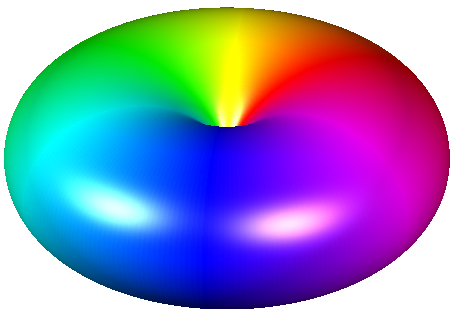
\includegraphics{../gfx/FM-spherical.pdf}};
    \node[inner sep=0] at (10, 0) {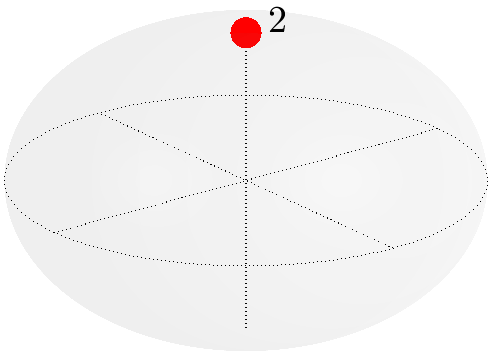
\includegraphics{../gfx/FM-Majorana.pdf}};
         
    % Colour bar
    \node[rotate=90] at (-5.5, 0) {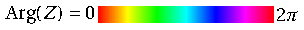
\includegraphics[scale=1.8]{../gfx/compiled_hsv.pdf}};
    \node at (16, 0) {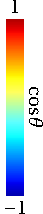
\includegraphics[scale=1.8]{../gfx/compiled_jet_majorana.pdf}};

    % FM lines
    \draw[->, dashed, line width=2] (0, 0.5) -- (0, 3);
    \node at (0, 3.5) {\LARGE \(\langle\hat{\vb{F}}\rangle\)};

    % Spinor label
    \node at (10, 3.7) {\LARGE \(\zeta^\text{FM} = (1, 0, 0)^T\)};
    % Labels
    \node at (0, -4) {\LARGE (a)};
    \node at (10, -4) {\LARGE (b)};

    % Orientation
    \draw[->, line width=2] (-4, -4) -- (-4, -3) node[above] {\LARGE \(z\)};
    \draw[->, line width=2] (-4, -4) -- (-3, -4) node[right] {\LARGE \(x\)};
    \draw[->, line width=2] (-4, -4) -- (-3.5, -3.5) node[right] {\LARGE \(y\)};

\end{tikzpicture}
\end{document}
